\section{Introduction}

\todo{Outline: first main result, then at the end follow sections with more details including design considerations}
The first quantum networks linking multiple quantum processors as end nodes have recently been realized as physics experiments in laboratories~\cite{moehring_2007_ion_traps,ritter_2012_elementary,hofmann_2012_heralded,stockill_2017_phasetuned,jing2019entanglement,stephenson_2020_highrate,pompili_2021_multinode,krutyanskiy_entanglement_2023} and fiber networks~\cite{liu2024creation,stolk2024metropolitan,knaut2024entanglement}, opening the tantalizing possibility of realizing advanced quantum network applications~\cite{wehner_2018_stages} such as data consistency in the cloud~\cite{benor_2005_byzantine}, privacy-enhancing proofs of deletion~\cite{poremba_quantum_2022}, exponential savings in communication~\cite{guerin_exponential_2016}, or secure quantum computing in the cloud~\cite{broadbent_2009_ubqc,childs_2005_secure_qc}. Demonstrations relied either on ad-hoc software, or chose to establish that hardware parameters were in principle good enough to support a given quantum network application, although the application itself was not realized~\cite{nadlinger_device-independent_2022,liu_2022_photonic_diqkd,zhang_2022_diqkd}.

It is a major challenge to design and implement an architecture that can enable the execution of arbitrary quantum network applications on quantum processors (\cref{qnodeos:fig:fig1}), while enabling programming in high-level software that neither depends on the underlying quantum hardware, nor requires the programmer to understand the physics of the underlying devices.  In the domain of the conventional internet, the possibility of programming arbitrary internet applications in high-level software has led to the realization of radically new communication applications by diverse communities, which had a transformative impact on our society~\cite{castells_impact_2013}. What's more, the advent of programmable hardware and new application areas sparked novel fields of computer science research and guided further hardware development.  A similar development is underway in quantum computing, where the availability of high-level programming tools allows a broad participation in developing applications~\cite{noauthor_quantum_2024}.

In realizing the first such architecture we overcome both fundamental challenges that are inherent to quantum network applications, as well as technological challenges that arise from the current state of the art of quantum network hardware.

\begin{figure}
\centering
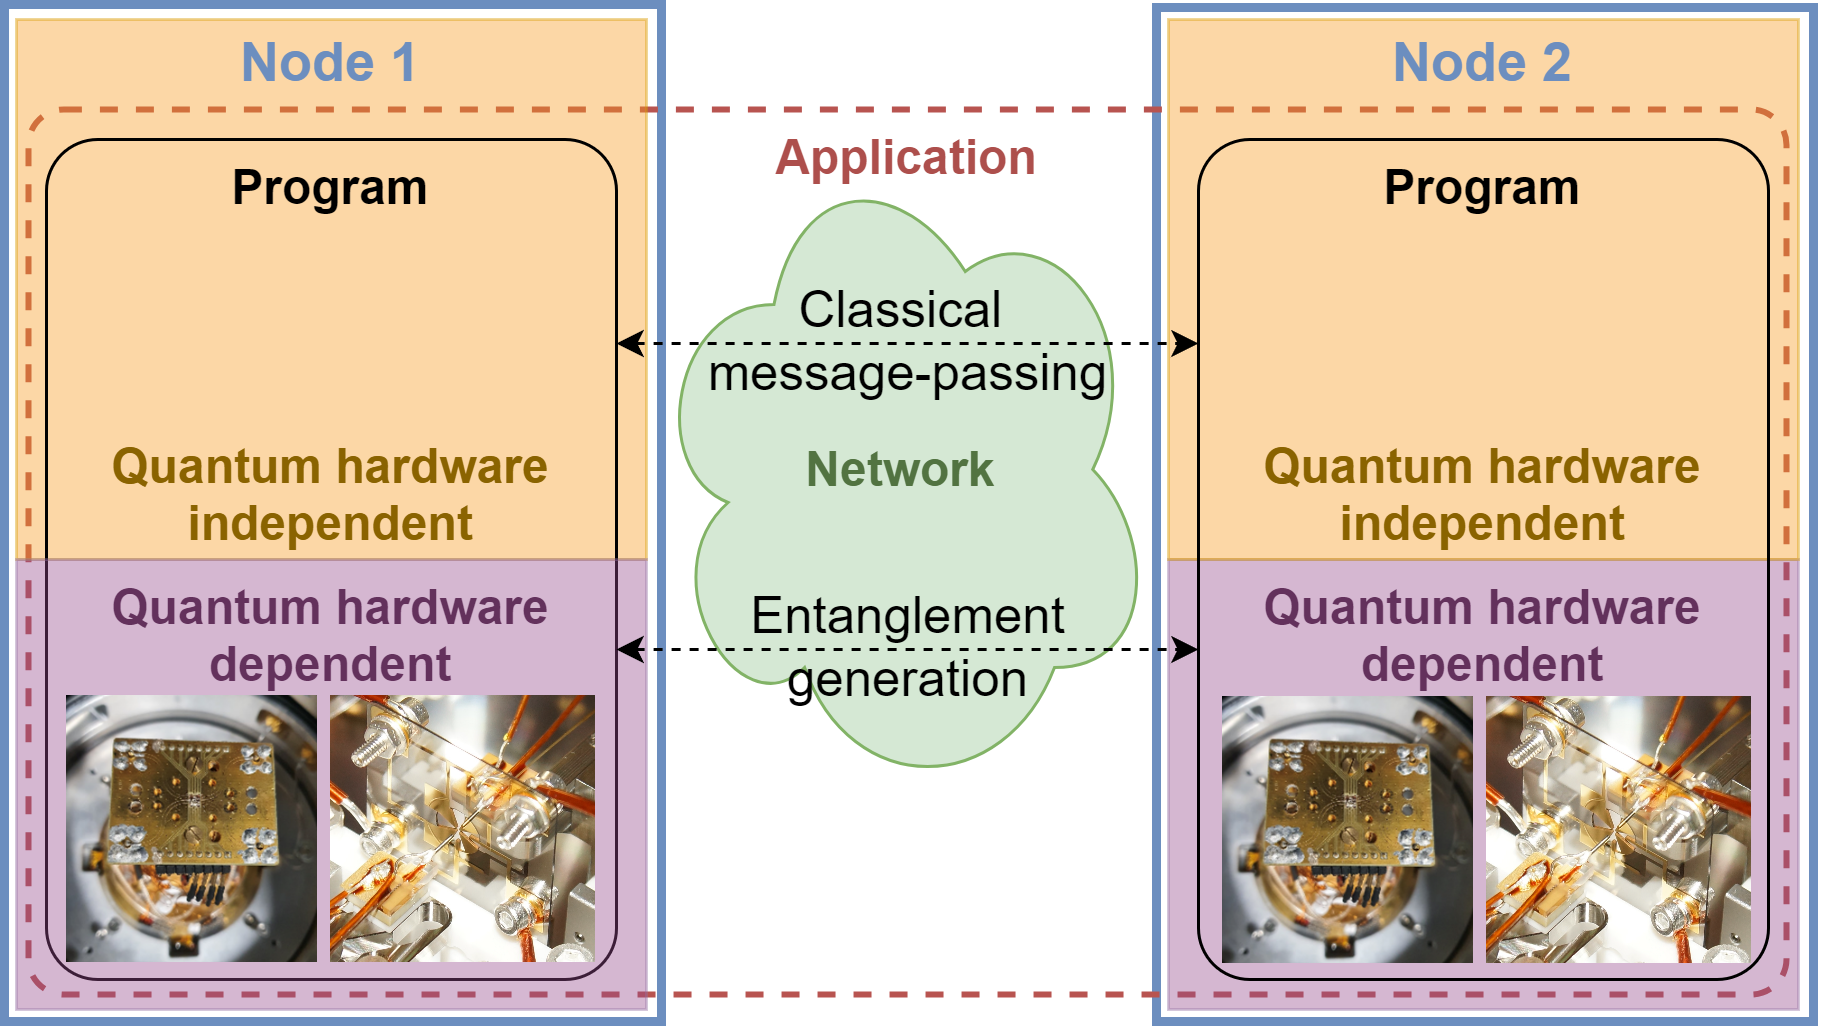
\includegraphics[width=1\linewidth]{figures/qnodeos/main/fig1/fig1.png}
\caption{\textbf{Application Paradigm.} A quantum networking application consists of multiple programs, each running on one of the end nodes~\cite{dahlberg_2022_netqasm} The distinct programs can only interact via (1) quantum communication (e.g. entanglement generation) and (2) classical communication. This allows a programmer to realize security-sensitive applications, but prohibits a global orchestration of the quantum execution, like one might do in (distributed) quantum computing~\cite{caleffi_distributed_2022} in which a single quantum program is executed on multiple nodes. Programs are written in high-level quantum hardware independent software, and executed on a quantum hardware independent system (our architecture) that controls a hardware dependent system (QDevice, \cref{qnodeos:fig:fig2}) such as a nitrogen-vacancy (NV) center node with a diamond chip (photo taken by authors, left images) or a trapped-ion quantum node~\cite{teller2023integrating} (right images). These platforms constitute physically very different QDevice systems, but can both be programmed by our architecture.}
\label{qnodeos:fig:fig1}
\end{figure}

\section{Design Considerations and Challenges}
\paragraph{Interactive Classical-Quantum Execution}
The execution of quantum network applications requires a continuing interaction between the quantum and classical parts of the execution, including interactions between different programs (\cref{qnodeos:fig:fig1}). For example, during secure quantum computing in the cloud~\cite{broadbent_2009_ubqc,ma_qenclave-practical_2022}, the program on the server is waiting for classical messages from a remote client before continuing the quantum execution at the server. This is in sharp contrast to quantum computing applications, where one quantum program can be executed in a single batch, without the need to keep quantum states live while waiting for input from other programs. In quantum computing, only relatively low-level interactions between classical and quantum processing are realized, such as in quantum error correction~\cite{lidar2013quantum}, or mid-circuit measurements~\cite{botelho_error_2022}. Higher-level classical-quantum interactions in quantum computing~\cite{bharti_noisy_2022} do not keep qubits live in memory.

We assume that the programs are divided into classical and quantum blocks of instructions (by a programmer or a compiler). Classical blocks consist of local classical operations executed on a conventional classical processor, as well as networked classical operations (i.e. sending messages to remote nodes) executed using network devices. Quantum blocks consist of local quantum operations (gates, measurements, classical control logic), as well as networked quantum operations (entanglement generation) executed on quantum hardware. A single quantum block, in essence, corresponds to a program in quantum computing, and may contain simple classical control logic, such as for the purpose of mid-circuit measurements~\cite{botelho_error_2022}.

\paragraph{Different Hardware Platforms}
Interfacing with different hardware platforms presents technological challenges: currently, a clear line between software and hardware has not been defined, and the low-level control of present-day quantum processor hardware has been built to conduct physics experiments. Early microarchitectures~\cite{bertels_quantum_2020,fu_2019_eqasm} and operating systems~\cite{giortamis_qos_2024,kong_2021_origin} for quantum computing do not address the execution of quantum network applications. We thus have to define a hardware abstraction layer (HAL), capable of interfacing with present-day quantum network setups. 

\paragraph{Timescales}
It is a fundamental challenge that different parts of such a system operate at vastly different timescales. For nodes separated by hundreds of kilometers, the duration of network operations is in the millisecond (ms) regime, and some applications~\cite{wehner_2018_stages} need  significant local classical processing (ms). In contrast, the time to execute quantum operations on processing nodes is in the regime of microseconds ($\mu$s), and the low-level control (including timing synchronization between neighboring nodes to generate entanglement~\cite{humphreys_2018_delivery}) requires nanosecond (ns) precision.

\paragraph{Memory Lifetimes}
Present-day quantum network nodes have short coherence times, posing a technological challenge to ensure operations are executed within the timeframe allowed by the quantum memory.

\paragraph{Scheduling Local and Network Operations}
In contrast to classical networking, entanglement is a form of stateful connection already at the physical layer where both nodes hold one qubit. Heralded entanglement generation requires agreement between neighboring network nodes to trigger entanglement generation in precise time-bins~\cite{dahlberg_2019_egp}, organized into a network schedule~\cite{skrzypczyk_2021_arch} that dictates when nodes make entanglement. It is a technological challenge to manage the interdependencies between the schedule of local operations, and the networked operations, since in all current processing node implementations~\cite{pompili_2021_multinode,drmota_robust_2023}, entanglement generation cannot be performed simultaneously with local operations~\cite{pompili_2021_multinode,krutyanskiy_light-matter_2019}. While interdependencies may be mitigated in the future~\cite{vardoyan_2022_netarch}, this implies that we cannot schedule (i.e. decide when to execute) the execution of local quantum operations independently of the network schedule.

\paragraph{Multitasking}
When executing quantum network applications, one node is typically idle while waiting for the other node before it can continue execution. It is hence a fundamental challenge how we can increase the utility of the system by performing multitasking~\cite{mccullough_design_1965-1,dennis_segmentation_1965}, that is, allowing the concurrent execution of several programs at once to make use of idle times. Consequently, there is a need for managing state and resources for multiple independent programs, including processes, quantum memory management, and entanglement requests. 

\begin{figure*}[htb]
\centering
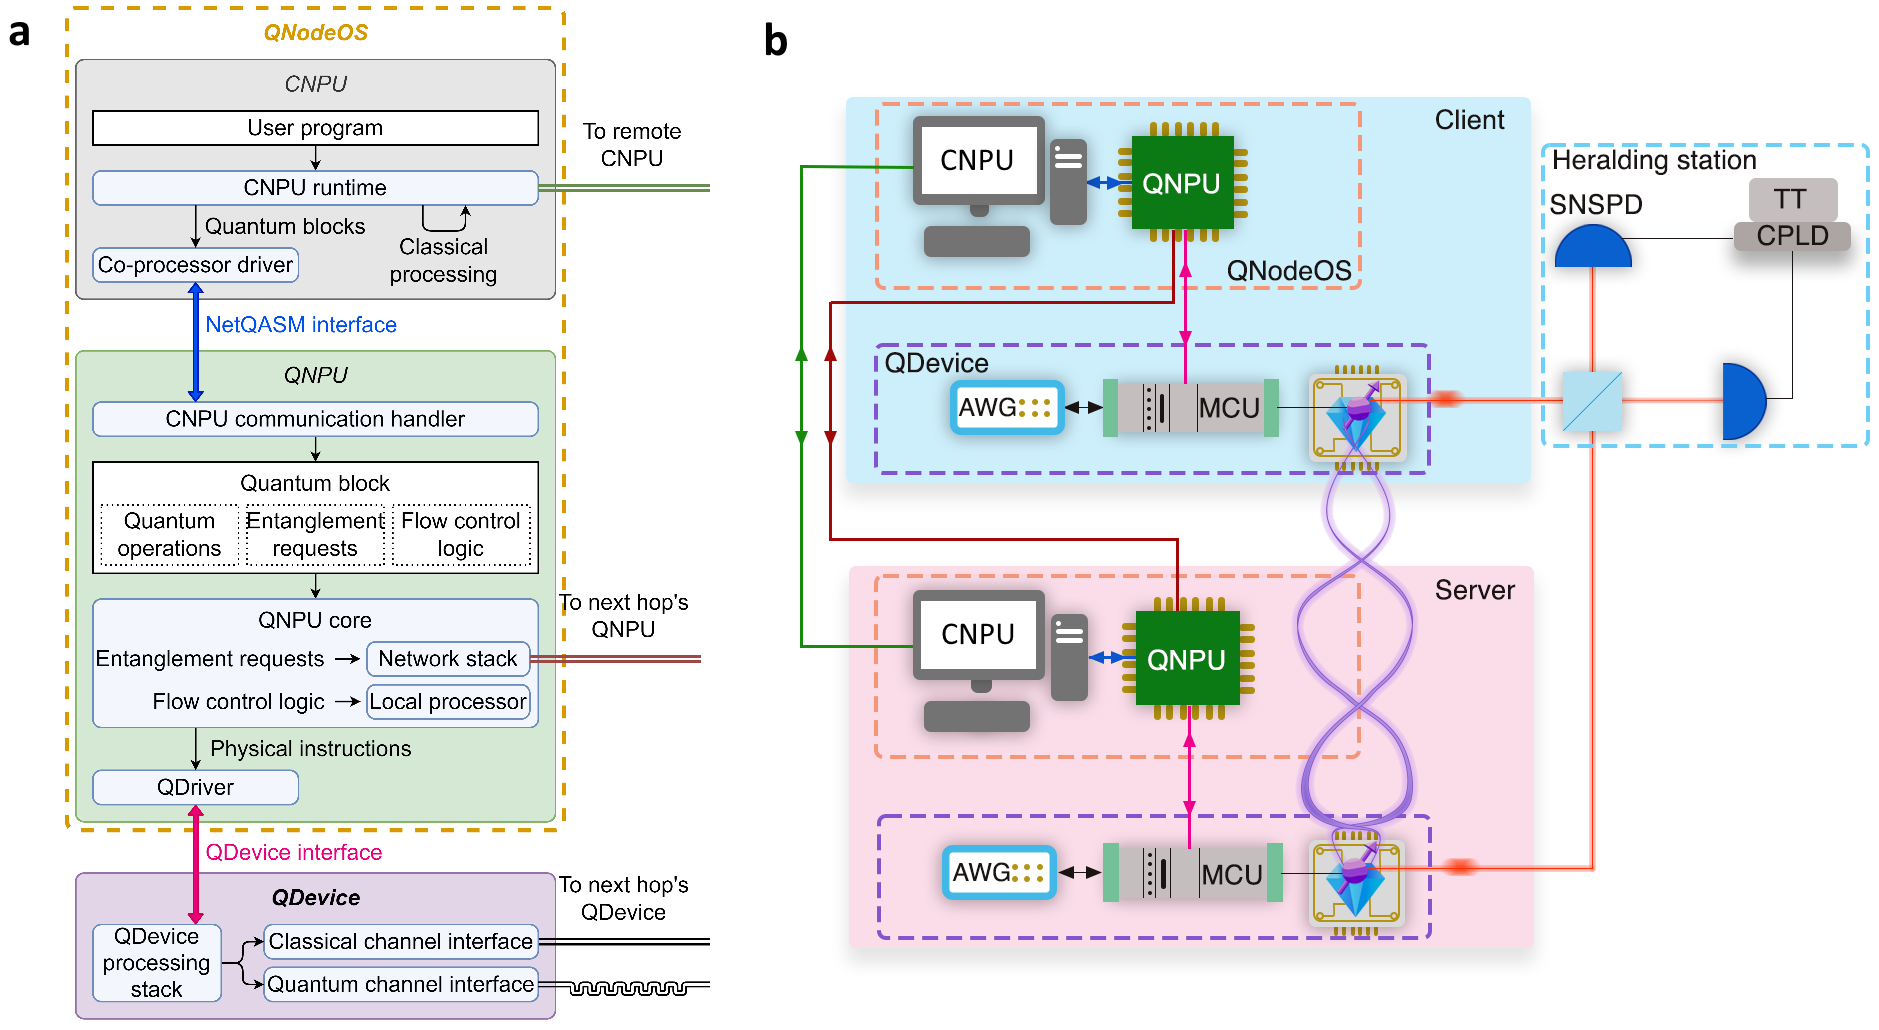
\includegraphics[width=1\linewidth]{figures/qnodeos/main/fig2/fig2.png}
\caption{\textbf{QNodeOS architecture.} \textbf{(a)} QNodeOS consists of a Classical Network Processing Unit (CNPU) and a Quantum Network Processing Unit (QNPU, classical system). QNodeOS controls a QDevice (quantum hardware and low-level classical control).
\textbf{(b)} Schematic of our implementation of QNodeOS on a two-node setup where both QDevices control a single qubit in a diamond nitrogen-vacancy (NV) center. The CNPU is implemented on a general-purpose PC, and the QNPU on an embedded system, connected via Gigabit Ethernet (blue). The QNPU connects to its QDevice via a serial peripheral interface (SPI, pink). The two QNPUs (brown), and the two CNPUS (green) connect to each other via Gigabit Ethernet. The setup is based on~\cite{pompili_2022_experimental} with two QDevices (including arbitrary waveform generators (AWG) and microcontroller units (MCU); QDevices communicating over a classical DIO interface) and a heralding station composed by a balanced 50:50 beam-splitter (whose output ports are connected to superconducting nanowire single-photon detectors (SNSPD) via optical fibers (red)),  a  TimeTagger (TT), and a \ac{CPLD} that heralds the entanglement generation between QDevices and sends a classical message to the MCU.}
\label{qnodeos:fig:fig2}
\end{figure*}

\section{Architecture}
\label{qnodeos:sec:architecture}
We divide the architecture logically into three main components (\cref{qnodeos:fig:fig2}, \cref{qnodeos:sec:methods}): The Classical Network Processing Unit (CNPU) is responsible for starting the execution of programs, and the execution of classical code blocks; the Quantum Network Processing Unit (QNPU) is responsible for governing the execution of the quantum code blocks; The CNPU and QNPU together form QNodeOS and control the QDevice, which is responsible for executing any quantum operations (gates, measurements, entanglement generation at the physical layer~\cite{dahlberg_2019_egp}) on the quantum hardware. Upon starting the execution the CNPU creates a corresponding CNPU process (a well-known concept in classical operating systems~\cite{dennis_programming_1966-1,tanenbaum_operating_2005}), registers the program on the QNPU (via the QNPU's end node application programming interface (API), \cref{qnodeos:sec:design:qnpu_stack}), which, in turn, creates its own associated QNPU process (including context such as process owner, ID, process state and priority). QNodeOS also defines kernel processes on the QNPU, which are similar to user processes, but are created when the system starts (on boot). The CNPU sends quantum blocks to the QNPU in the form of NetQASM subroutines~\cite{dahlberg_2022_netqasm}. Classical control logic in quantum blocks is executed by the QNPU processor. Quantum gates and measurements (from any QNPU process) and entanglement instructions (from the network process) are delegated to the QDevice by submitting physical instructions (\cref{qnodeos:sec:methods}), after which the QDevice responds back with the result of the instruction. 

To enable different hardware platforms, we introduce a QDriver realizing the HAL for any hardware corresponding to our minimal QDevice system model (\cref{qnodeos:sec:methods}). The QDriver is responsible for translating quantum operations, expressed in NetQASM~\cite{dahlberg_2022_netqasm}, into platform dependent (streams of) physical instructions to the underlying QDevice. We realize a QDriver for the trapped-ion system of~\cite{teller2023integrating,teller2021heating}, and one for NV centers in diamond based on the system of~\cite{hermans2022qubit,pompili_2021_multinode,pompili_2022_experimental}. We validate the trapped-ion QDriver (\cref{qnodeos:fig:fig5}) by implementing and verifying a set of single-qubit gate operations (\cref{qnodeos:sec:methods}), and the QDriver on the NV system as part of the full stack system evaluation (see below). 
To allow for different timescales, we logically divide the architecture into CNPU, QNPU and QDevice which can thus be realized at different timing scale granularities. In our proof-of-concept implementation, we realize the CNPU and QNPU on different devices, reflecting the ms timescales of communication between distant nodes (\cref{qnodeos:sec:methods}).

Ensuring the necessary interactivity requires architectural as well as implementation choices: as programs may depend on messages from remote nodes, the architecture needs to be able to dynamically handle both classical and quantum blocks, even if not known at runtime. Consequently, it is not possible to preload all quantum blocks of the program into the low-level controller of the QDevice ahead of time as done in previous physics experiments. Instead, in our system model the QDevice is capable of executing individual physical instructions similar to a classical CPU. Consequently, the QNPU is continuously ready to receive new NetQASM subroutines from the CNPU, and the QDevice can continuously receive and respond to physical instructions from the QNPU (\cref{qnodeos:sec:methods}).

In our NV QDevice implementation, we address the challenge of interactivity by interleaving specific preloaded pulse sequences (realizing physical instructions sent from QNodeOS) and dynamical decoupling (DD) sequences (protecting quantum memory from decoherence) in an arbitrary waveform generator (AWG)~\cite{zurich_instruments_hdawg_2019}. The DD sequences extend qubit coherence times up to $T_{\text{coh}} = 13(2)$ ms, while arbitrary physical instructions can be handled by triggering the corresponding pulse sequence, without knowing them in advance (\cref{qnodeos:sec:methods}).

To integrate local operations with the network schedule, our architecture first introduces a QNPU scheduler that can choose which of the ready processes is assigned to the local processor (\cref{qnodeos:fig:fig2}) and QDevice. This allows interleaving the execution of different processes directly on the QNPU without incurring delays on the timescale of the CNPU (ms), addressing the challenge of short coherence times. In our implementation, we choose to schedule QNPU processes using a priority based non-preemptive scheduler~\cite{liu_1973_scheduling}, due to limited quantum memory lifetimes, which make it undesirable to pre-empt and temporarily store quantum states while halting the execution. Second, we realize a network process as a kernel process, which manages entanglement generation using the network stack~\cite{dahlberg_2019_egp,kozlowski_2020_qnp} (implemented in~\cite{pompili_2022_experimental} without the ability to execute network applications), including a network schedule that can be determined by a time-division multiple access (TDMA) controller~\cite{skrzypczyk_2021_arch}. The network process handles entanglement requests submitted by user processes, coordinates entanglement generation with the rest of the network via the TDMA controller, interacts with the QDevice and eventually returns entangled qubits to user processes. User processes enter the waiting state when they need entanglement, and become ready again once entanglement was delivered. The network process has the highest scheduling priority, and is consequently given precedence over the execution of any local quantum operations. We remark local operations may still be executed during time-bins already occupied by the network schedule, if a running non-preemptable user process prevents the network process from running, as we indeed observe in our evaluation.

To increase utility, QNodeOS allows multiple programs to be run concurrently, using the QNPU scheduler from above to enable multitasking~\cite{mccullough_design_1965-1,dennis_segmentation_1965} user processes on the QNPU itself. The QNPU hence needs to keep context for each process, including a virtual quantum memory space (as in classical operating systems~\cite{daley_virtual_1968-1}). Similar to classical memory management systems~\cite{peterson_operating_1985}, a quantum memory management unit (QMMU) on the QNPU manages qubit allocations from processes, and translates virtual qubit addresses in NetQASM subroutines to physical addresses in the QDevice. This allows flexibility in translating a virtual qubit address to: (1) a different physical qubit address over time, allowing qubits to be rearranged transparently in the physical memory in the future, or (2) a logical qubit address, when QNodeOS is executed on top of a processor employing quantum error correction~\cite{lidar2013quantum}. Entanglement generation between different pairs of processes at remote nodes are distinguished by Entanglement Request (ER) sockets, inspired by classical sockets~\cite{chesson_network_1975-1,leach_architecture_1983}, which are established once a user process requests entanglement from the network process. In our implementation, processes of the same priority are scheduled first-come-first-served~\cite{peterson_operating_1985}, where the total schedule of the program in our implementation is dependent both on the schedule on the CNPU as well as the QNPU (\cref{qnodeos:sec:methods}).

\begin{figure*}[htbp]
\centering
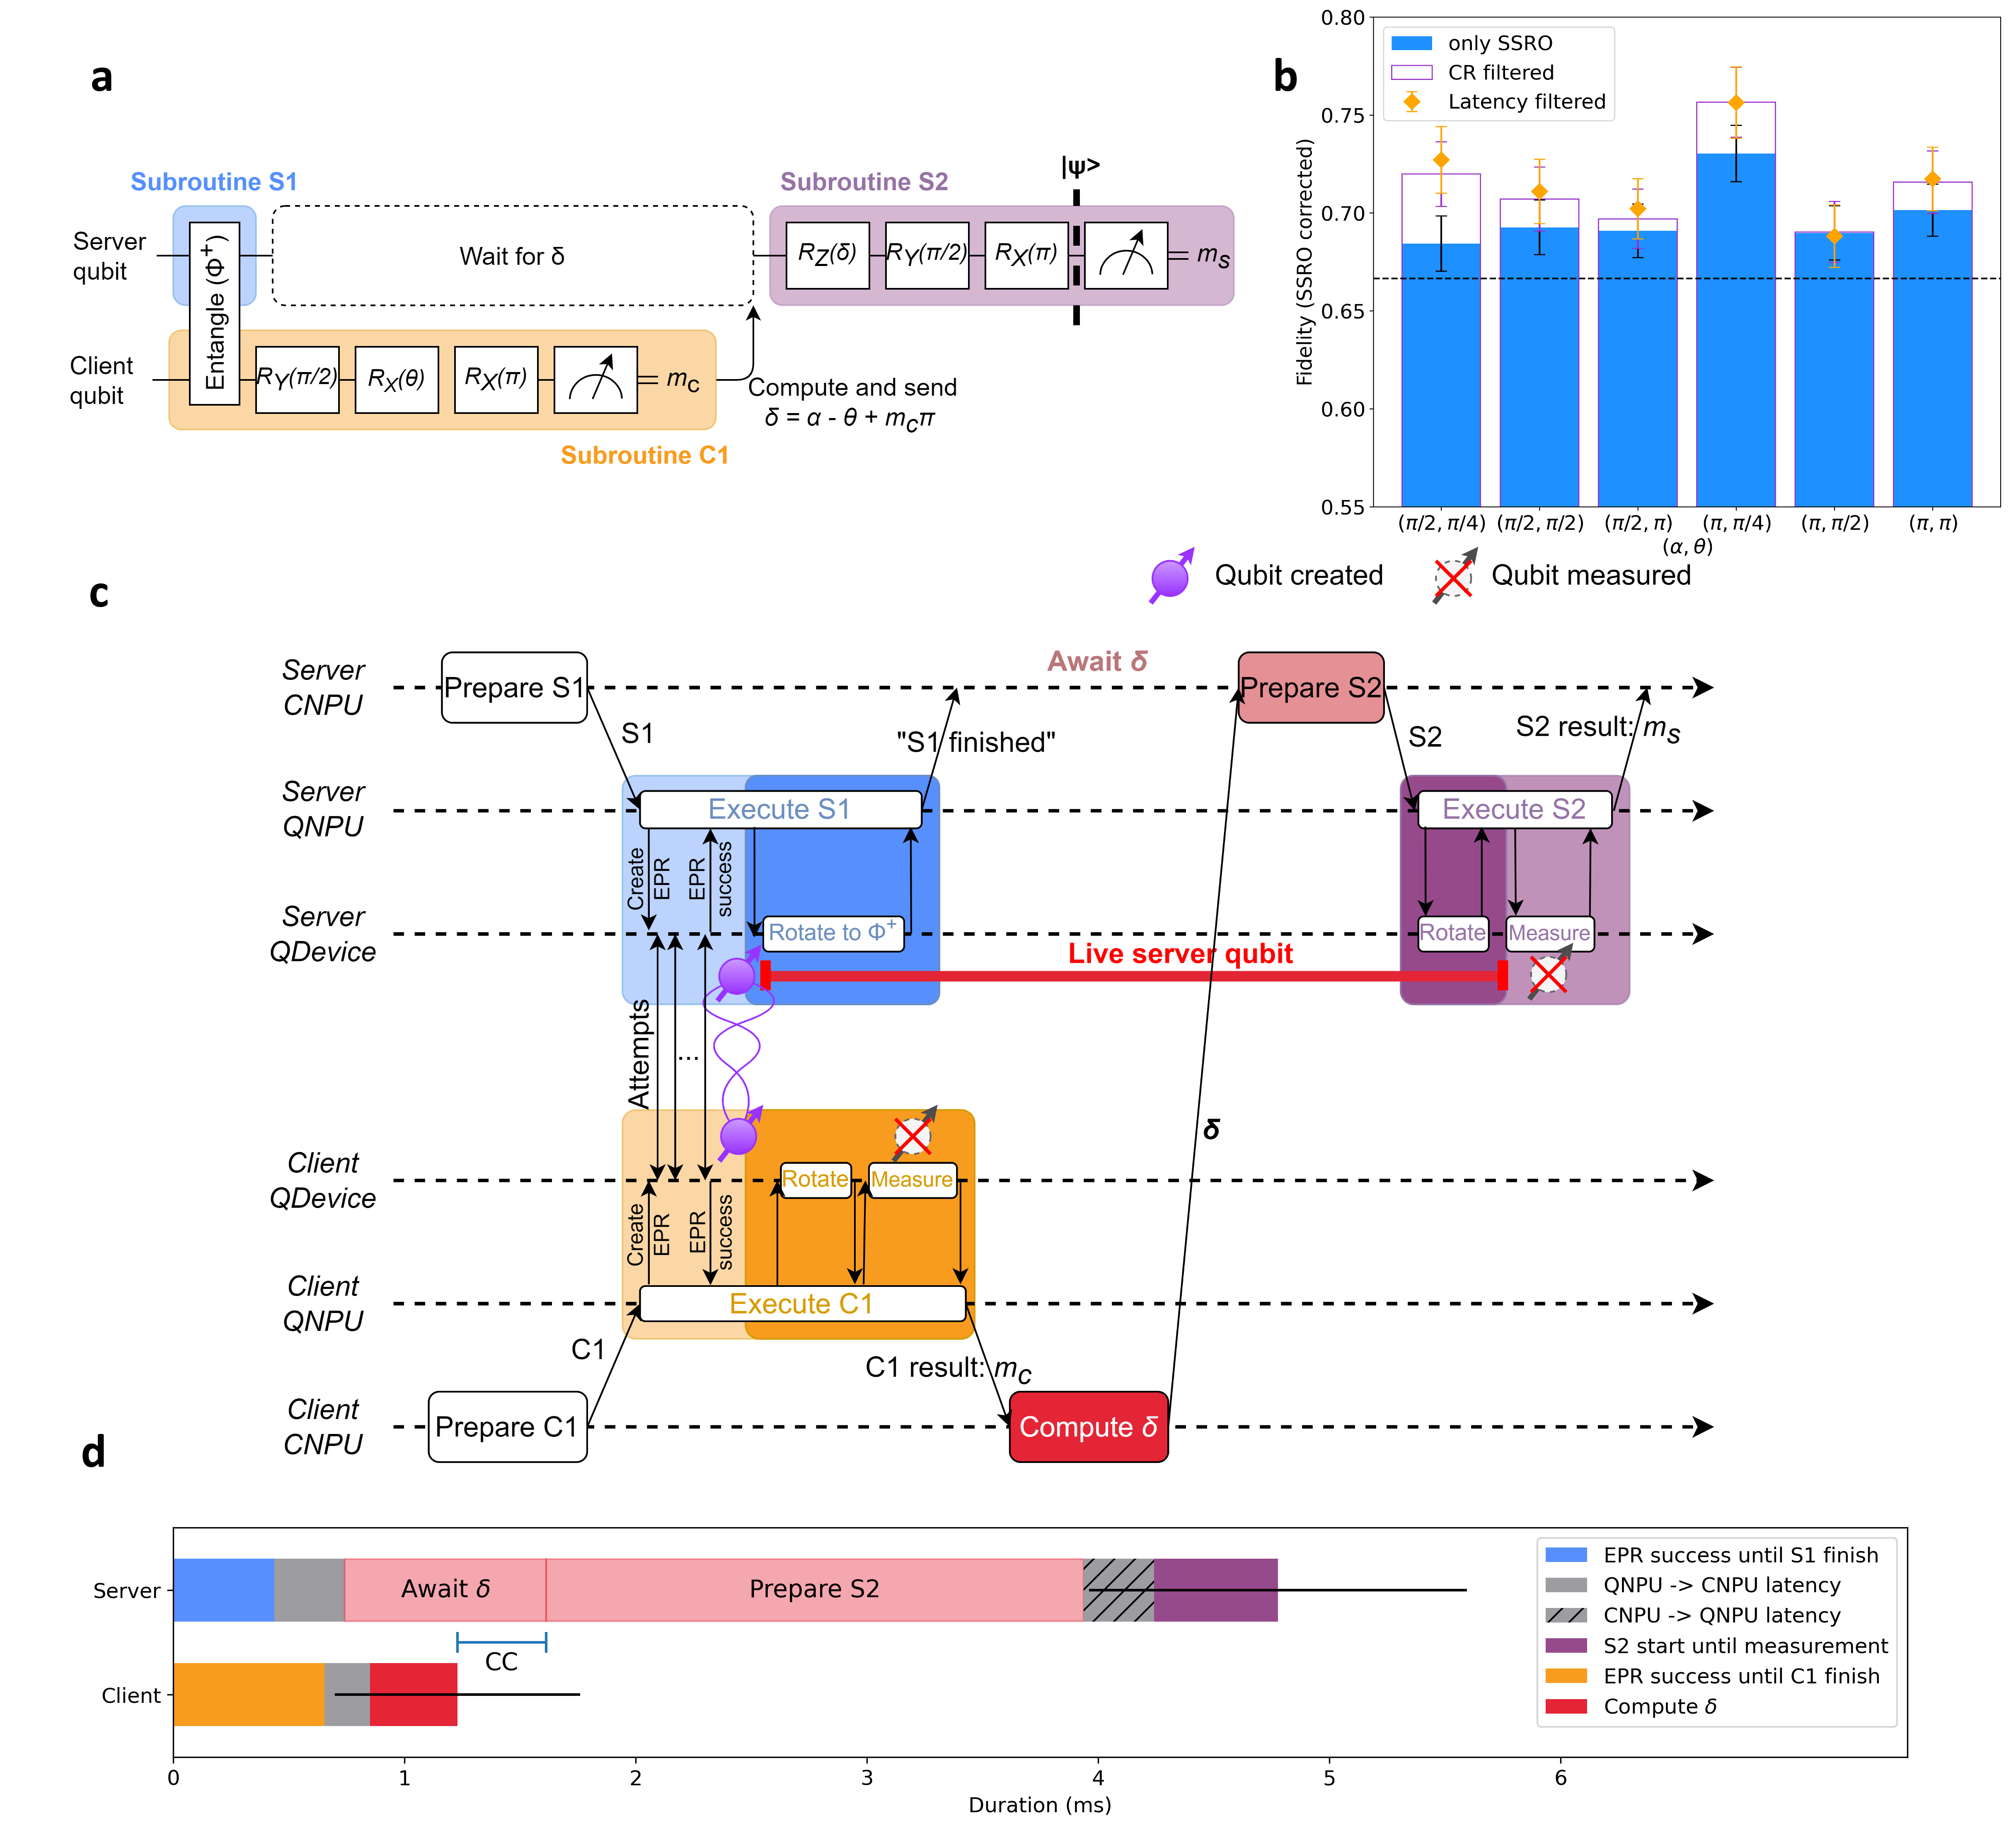
\includegraphics[width=0.89\linewidth]{figures/qnodeos/main/fig3/fig3.png}
\caption{\textbf{Delegated computation between two NV center nodes using QNodeOS.} 
\textbf{(a)} Delegated Quantum Computation (DQC) circuit (effective computation: single-qubit rotation $R_Z (\alpha)$, \cref{qnodeos:sec:methods}). The DQC application consists of $k$ repetitions of this circuit (varying measurement bases for tomography on $\ket{\psi}$) realized by two programs: the DQC-client program (client node, repeating the sequence ``quantum block (C1, orange) – classical block (computing $\delta$)'' $k$ times), and the DQC-server program (server node, repeating ``quantum block (S1, blue) - classical block (receiving $\delta$) – quantum block (S2, purple)'' $k$ times). Client and server produce an entangled pair $\ket{\Phi^+} = (\ket{00} + \ket{11}) / \sqrt{2}$ (S1 and first part of C1). The client performs local gates and a measurement (``destroying'' qubit), resulting in outcome bit $m_c$ (rest of C1). Client computes $\delta$ as function of $m_c$ and DQC parameters $\alpha \in [0,2\pi)$ and $\theta \in [0, 2\pi)$, and sends $\delta$ to server (classical message). Meanwhile the server keeps its qubit coherent (alive). Upon receiving $\delta$, the server applies gates depending on $\delta$, resulting in single-qubit state $\ket{\psi}$ (S2) depending only on $\alpha$ and $\theta$.
\textbf{(b)} Experimental results of executing DQC for 6 different sets of $(\alpha, \theta)$ parameters ($k=1200$, i.e. 7200 executions of the circuit of~\ref{qnodeos:fig:fig3}a). The fidelity of the resulting server state to the target state $\ket{\psi}$ is estimated using single-qubit tomography (1200 measurement results per data point), and corrected for known tomography errors (SSRO, blue), and post-selected for Charge-Resonance (CR) check validation (purple), and post-selected for latencies (orange) (\cref{qnodeos:sec:methods}).
\textbf{(c)} Sequence diagram including the interaction CNPU-QNPU-QDevice for one execution of the DQC circuit of \ref{qnodeos:fig:fig3}a on QNodeOS (repeated $k=1200$ times in each experiment) (time flows to the right; not to scale). CNPUs prepare NetQASM subroutines (C1, S1, S2), and send them to their respective QNPUs. CNPUs also do classical computation (computing $\delta$) and communication (message containing $\delta$). QNPUs execute subroutines, sending physical instructions to their QDevices. Entanglement is generated by QDevices doing a batch of attempts, resulting in the heralding of a two-qubit entangled state (Bell pair) rotated to $\ket{\Phi^+}$ by the server.
\textbf{(d)} Processing times and latencies while server qubit is live (time frame red line 3c, averaged over all 7200 circuit executions except executions with latency spikes, see~\cref{qnodeos:sec:methods}), including CNPU-QNPU communication latencies, CNPU processing on both nodes and client-server communication latency (CC) (average total of $\sim 4.8 (\pm 0.8)$ ms, error bars for the sum of individual segments (variance per segment in~\cref{qnodeos:sec:processing_time_latencies}).}
\label{qnodeos:fig:fig3}
\end{figure*}


\section{Demonstrations}
\paragraph{Delegated Computation}
We first validate our architecture and implementation by the first successful execution of an arbitrary – i.e. not preloaded – execution of a quantum network application in high-level software on quantum processors. We implement QNodeOS on a two-node setup of NV centers using one qubit per node (\cref{qnodeos:fig:fig2}, \cref{qnodeos:sec:methods}). We choose to execute an elementary form of delegated quantum computation (DQC)~\cite{broadbent_2009_ubqc} from a client to a server, because the client and server programs jointly realize repetitions of a circuit (\cref{qnodeos:fig:fig3}a) that triggers all parts of our system (\cref{qnodeos:fig:fig3}c). 
We first verify that the quantum result (fidelity) was found to be above the classical bound~\cite{massar_optimal_1995} $> 2/3$, which verifies that QNodeOS can successfully handle interactive applications consisting of entanglement generation, millisecond-scale memory lifetimes, and classical message passing. The non-perfect fidelity (\cref{qnodeos:fig:fig3}b) comes mainly from two sources: a noisy entangled state with fidelity 0.72(2) (quantum hardware limitation), and decoherence in the server qubit (depending on $T_{\text{coh}}$) due to waiting for several milliseconds (classical software latencies, \cref{qnodeos:fig:fig3}d).
We proceed to characterize latencies. As expected, we find that the duration that the server qubit must remain alive is dominated (> 50\%) by processing in the CNPU, which could be improved by caching the preparation of S2, and implementing the CNPU and QNPU on one board (Outlook). We observe that CNPU processing time varies significantly (standard deviation 30\%, \cref{qnodeos:sec:processing_time_latencies}), due to limited scheduling control over CNPU processes (\cref{qnodeos:sec:methods}).  Using an a priori estimate of what delays lead to too low a quality of execution (i.e. delays that are too long for the server qubit to be stored with sufficiently high quality), we discard application iterations in which the CNPU latencies spiked by more than 8.95 ms. This lead the discarding of 2\% of iterations in post-processing (\cref{qnodeos:sec:methods}).

\paragraph{Demonstration of Multitasking}
We also validate QNodeOS's multitasking capability by the first concurrent execution of two quantum applications on a quantum network: the DQC application, and a single-node local gate tomography (LGT) application on the client (\cref{qnodeos:fig:fig4}a). The two programs for the client are started in the CNPU at the same time (two CNPU processes, subject to CNPU scheduler), which means that the QNPU continuously receives subroutines for both programs from the CNPU (two QNPU processes and corresponding subroutines, subject to QNPU scheduler). This leads to a multitasking challenge directly on the QNPU to schedule the different subroutines received (\cref{qnodeos:fig:fig4}b). Since the client has only one qubit, the multitasking of DQC and LGT never results in both programs having a quantum state alive on the client; therefore, multitasking should not affect the fidelity of LGT. We observe interleaved execution of DQC quantum blocks and LGT quantum blocks on the client node (\cref{qnodeos:fig:fig4}b). The LGT application produces a quantum result (fidelity, \cref{qnodeos:fig:fig4}c) equal to that in the scenario where we run LGT on its own (not interleaved by DQC circuit executions), as expected.

We further test multitasking by scaling up the number of programs executed concurrently, up to 5 DQC and 5 LGT programs running on the client at the same time. The interleaved execution of subroutines of different programs increases device utilization (fraction of time spent on executing physical instructions) on the client QDevice compared to the same scenario but with multitasking disabled (\cref{qnodeos:fig:fig4}d). As expected, we observe that LGT subroutines were scheduled to be executed in between DQC subroutines, resulting in lower client QDevice idle time. When multitasking 1 DQC and 1 LGT program, we observe 1 or 2 subroutines in between DQC iterations in most cases (LGT subroutine duration ~2.4 ms, \cref{qnodeos:sec:multitasking-scaling}). We observe cases where both server and client QDevice remain idle, which could be improved in part by smarter CNPU-QNPU scheduling algorithms: (1) both the client and server wait until the start of the next network schedule time-bin (time-bin length 10 ms) (2) the client QNPU finishes a subroutine for user process P, but must wait until the CNPU sends the next subroutine for P (up to 150 ms for 1 DQC and 1 LGT program, but less (up to only 8 ms) when more applications are running, since there are more CNPU processes independently submitting subroutines), (3) the client is ready to perform entanglement generation for DQC, but the next time-bin starts only at some future time $t$, preventing activation of the network process. The scheduler activates a user process which runs a LGT circuit, which completes at some time $>t$, delaying the start of the DQC network process, even though the server node was ready at $t$.

\begin{figure*}[htbp]
\centering
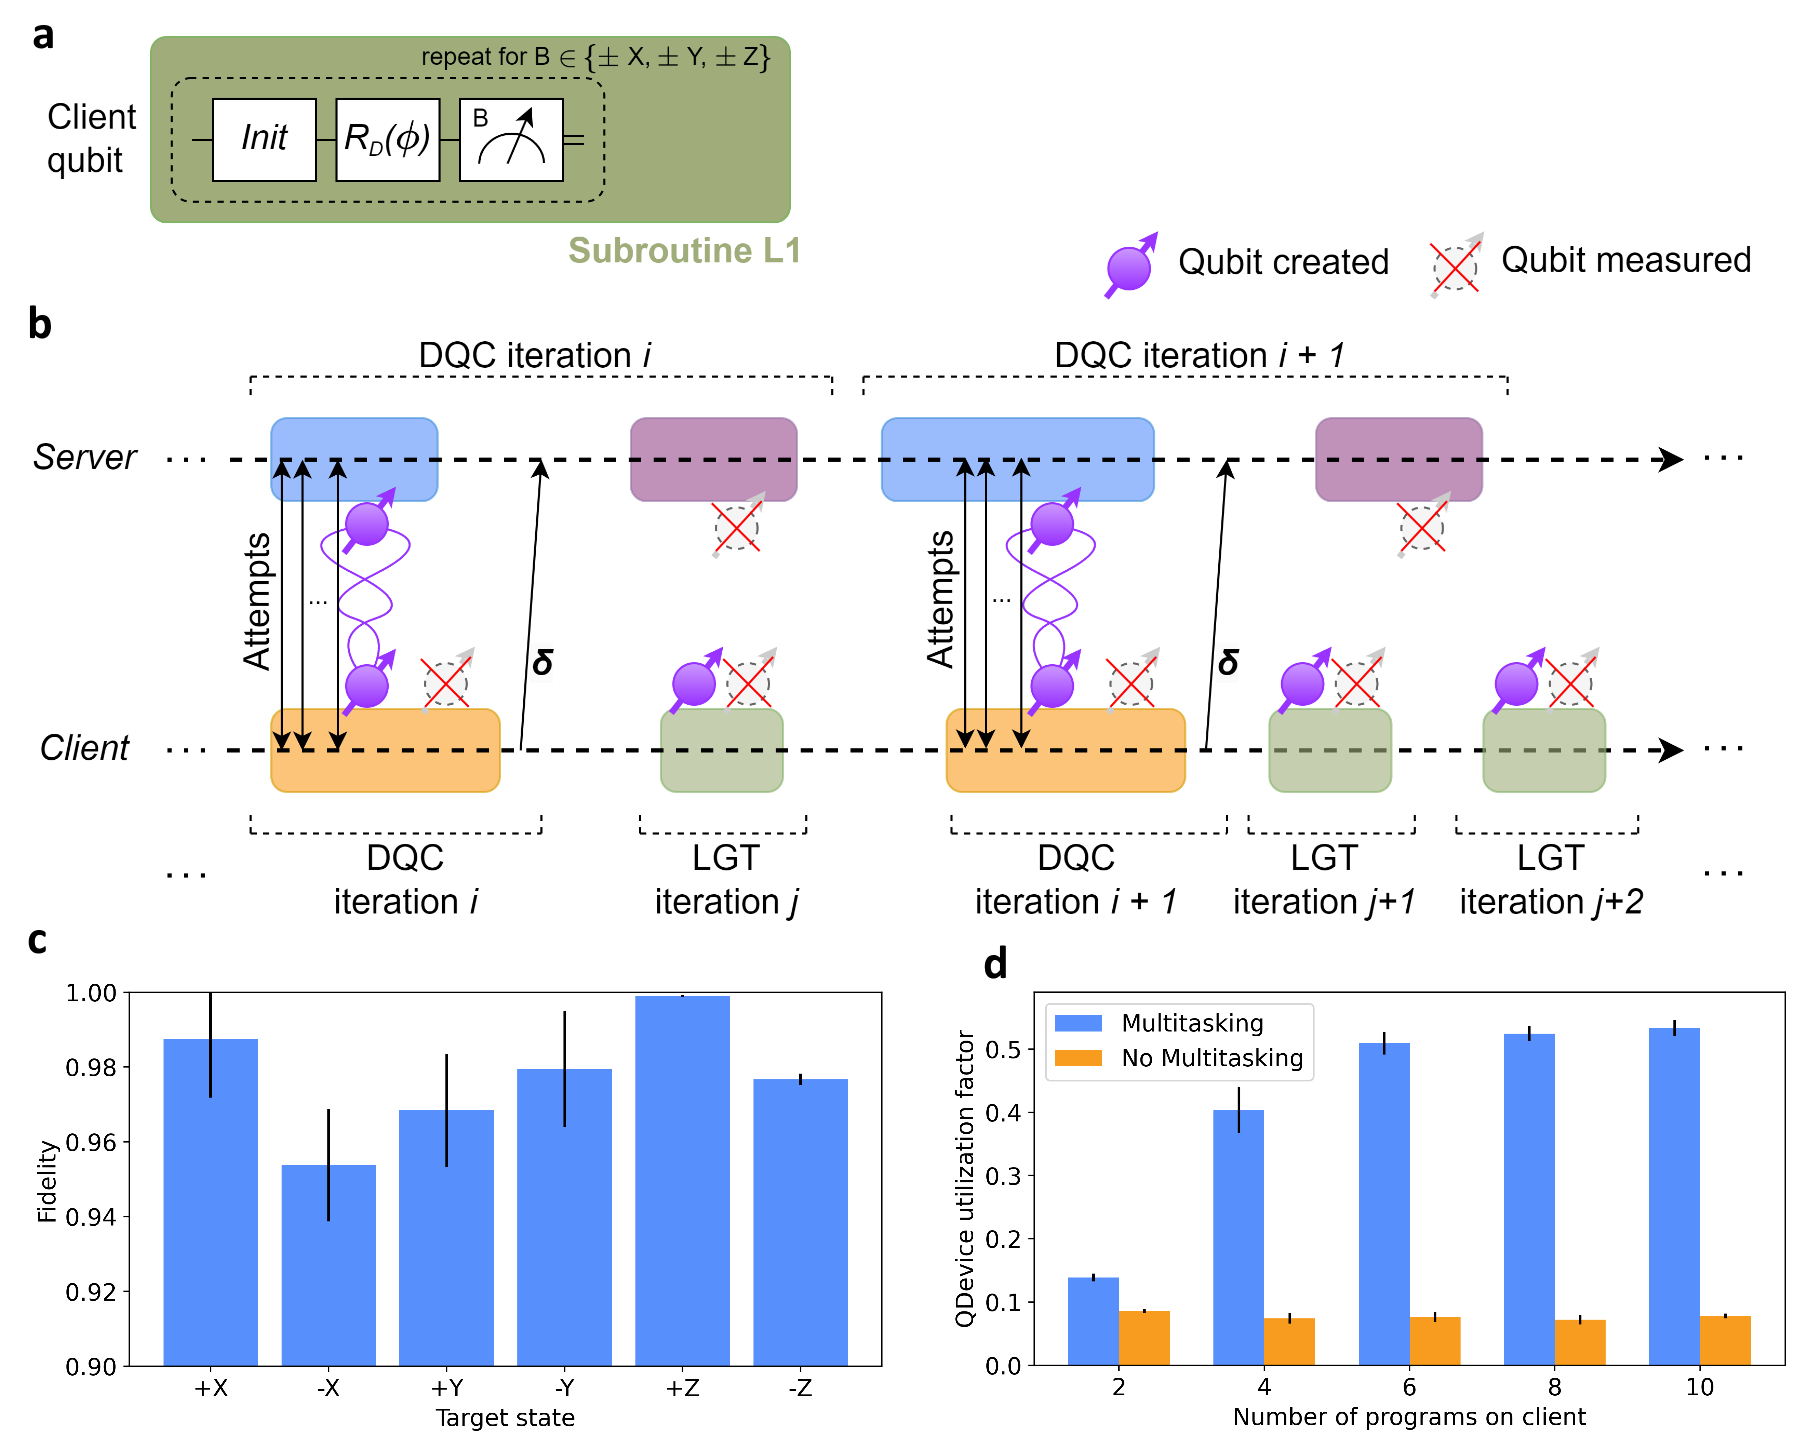
\includegraphics[width=0.95\linewidth]{figures/qnodeos/main/fig4/fig4.png}
\caption{\textbf{Multitasking experiment on two NV centers with QNodeOS}.
\textbf{(a)} Local Gate Tomography (LGT) Circuit. A single NetQASM subroutine (L1) executes the following 6 times for different bases $B \in \{\pm X, \pm Y, \pm Z\}$: initialize qubit to $\ket{0}$, rotate around fixed axis $D \in \{X,Y\}$ by angle $\ket{\phi}$, measure in $B$. The LGT application consists of a single LGT program, which submits subroutine L1 for execution to the QNPU (fixed $D$ and $\phi$) $k$ times in succession.
\textbf{(b)} Example sequence diagram illustrating concurrent execution (multitasking) of the DQC application (\cref{qnodeos:fig:fig3}) and the LGT program on the client: time slice in which two DQC circuit repetitions (\cref{qnodeos:fig:fig3}a) are realized (2 subroutines on the client (orange), 4 on the server (blue and purple)), and three LGT circuit repetitions (3 subroutines, green). The client QNPU receives subroutines for both the DQC program and the LGT program, which the QNPU scheduler can interleave: While the server executes S2 (purple), the client cannot yet execute the next S1 (orange) since it involves joint entanglement generation. In this idle time, the client can execute a number of LGT subroutines (number can vary).
\textbf{(c)} Results of multitasking LGT (client) and DQC (on both server and client). For each input pair $(D, \phi) \in \{ (X,0), (X,\pi), (Y,pi/2), (Y,-\pi/2), (X,-\pi/2), (X,\pi/2) \}$ (6 cardinal states $\{\pm X, \pm Y, \pm Z\}$), the following experiment was performed: simultaneously (1) a single LGT program was initiated on the client ($k=1000$), (2) a single DQC-client program was initiated on the client ($k=200$ successive subroutines), and (3) a single DQC-server program was initiated at the server ($k=200$, i.e. 400 successive subroutines). This resulted in a total of 6000 LGT subroutine executions and 36000 LGT measurement results, yielding plotted fidelity estimates for the LGT quantum state before measurement. Results are the same as running LGT on its own (no multitasking with DQC), as expected (\cref{qnodeos:sec:multitasking-tomography}).
\textbf{(d)} Scaling number of programs on the client. For $N \in \{1,2,3,4,5\}$, we initiate at the same time: (1) $N$ LGT programs (each using $k=100$) on the client, (2) N DQC-client programs on the client (each using $k=60$), and (3) $N$ DQC-server programs on the server (each using $k=60$). This results in $2N$ programs active at the same time on the client, each continuously submitting subroutines from the CNPU to the QNPU, where the QNPU scheduler chooses which process to execute when. Each experiment was repeated but with multitasking disabled on the client. Plot shows the utilization factor of the QDevice (fraction of time spent executing instructions), corrected for variable entanglement generation duration (\cref{qnodeos:sec:methods}), with (blue) and without (orange) multitasking, showing that multitasking can increase device utilization.}
\label{qnodeos:fig:fig4}
\end{figure*}

\section{Outlook}
We designed and implemented the first architecture allowing high-level programming and execution of quantum network applications. To deploy our system onto nodes separated by several kms it would be desirable to merge both the CNPU and the QNPU onto one system board, ideally with mutual access to a shared memory to avoid ms delays in their communication. Such a merge would also allow the definition of a joint classical-quantum executable and processes, opening further doors to reduce latencies by a better scheduling control.

Our work provides a framework for a new domain of computer science research into programming quantum network applications on quantum processors including: novel real-time~\cite{ramamritham_scheduling_1994} scheduling algorithms for classical-quantum processes, compile methods for quantum network applications, or novel programming language concepts including entanglement to make software development even easier, thus advancing the vision to make quantum network technology broadly available.


\begin{figure}[htb]
\centering
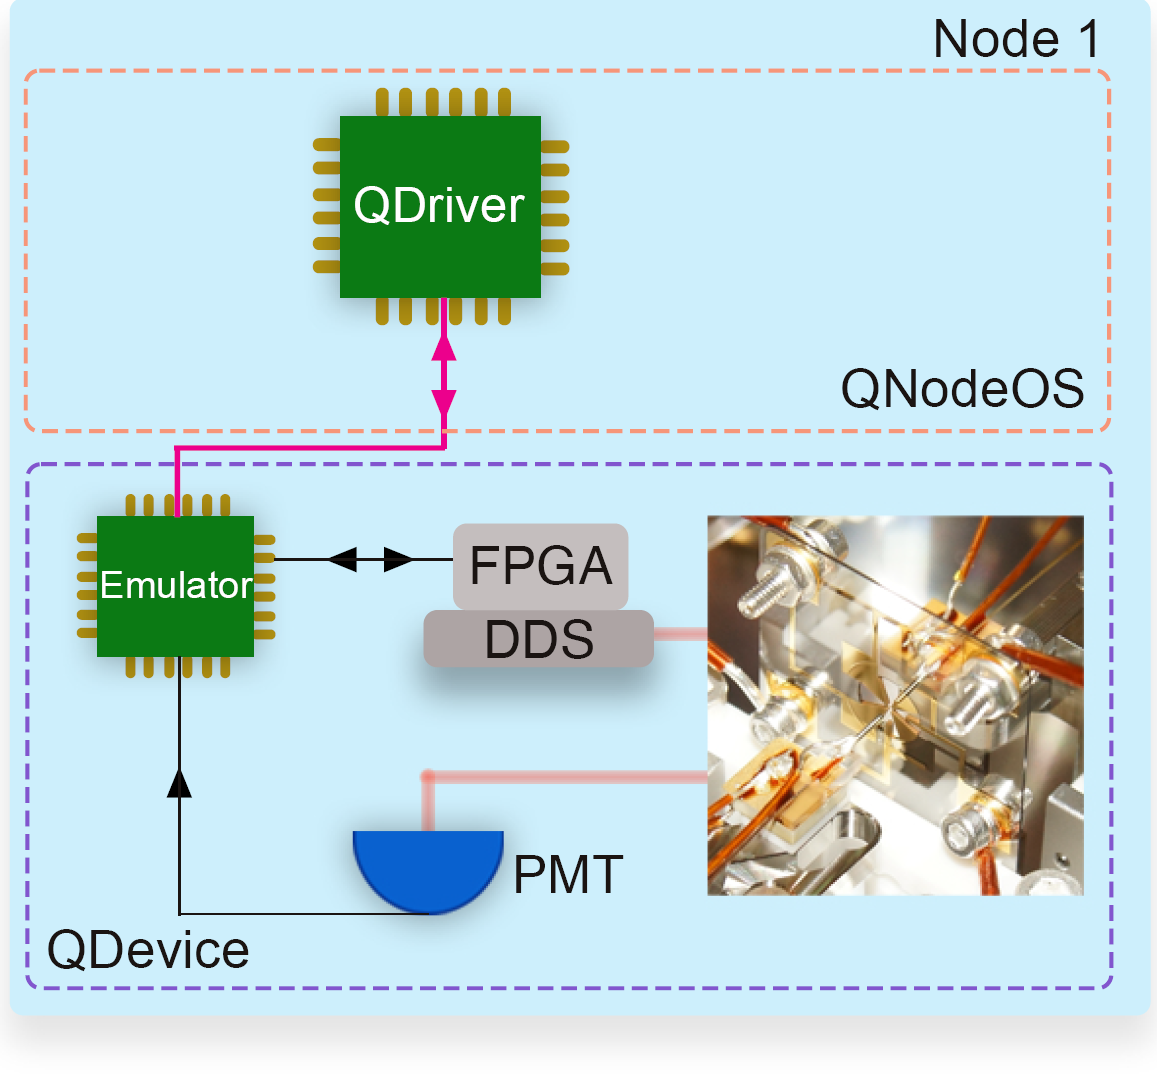
\includegraphics[width=1\linewidth]{figures/qnodeos/main/fig5/fig5.png}
\caption{\textbf{Trapped-ion QDevice implementation.} Schematic of our implementation of QNodeOS on a single-node setup in which the QDevice contains a single trapped-ion qubit. The QNPU QDriver is implemented on a field-programmable gate array (FPGA) that connects to its QDevice via a serial peripheral interface (SPI) (\cref{qnodeos:sec:methods}). The setup consists of an emulator that translates between SPI messages and TTL signals, experimental control hardware that includes an FPGA and direct digital synthesis (DDS) modules, a trapped-ion qubit~\cite{teller2023integrating} under ultra-high vacuum (\cref{qnodeos:fig:fig1}), and a photomultiplier tube (PMT) that registers atomic fluorescence.}
\label{qnodeos:fig:fig5}
\end{figure}